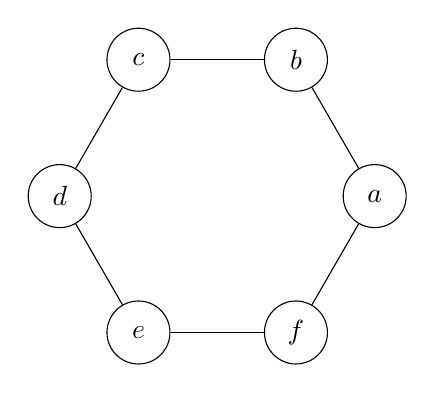
\begin{tikzpicture}

\node[draw, circle, minimum size=0.8cm] (a) at (0:2) {$a$};
\node[draw, circle, minimum size=0.8cm] (b) at (60:2) {$b$};
\node[draw, circle, minimum size=0.8cm] (c) at (120:2) {$c$};
\node[draw, circle, minimum size=0.8cm] (d) at (180:2) {$d$};
\node[draw, circle, minimum size=0.8cm] (e) at (-120:2) {$e$};
\node[draw, circle, minimum size=0.8cm] (f) at (-60:2) {$f$};

\draw (a) -- (b);
\draw (b) -- (c);
\draw (c) -- (d);
\draw (d) -- (e);
\draw (e) -- (f);
\draw (f) -- (a);
\end{tikzpicture}